\documentclass[a4paper, 11pt, onecolumn, openany, titlepage]{report}
\usepackage[utf8]{inputenc}
\usepackage{enumitem}
\usepackage{filecontents}
\usepackage[T1]{fontenc}
\usepackage{url}
\usepackage{breakcites}
\usepackage{graphicx}
\graphicspath{{qualitative-results/}{quantitative-results/}}
\usepackage{caption}
\usepackage{subcaption}
\usepackage{titlesec}
\usepackage{tabularx}
\usepackage{afterpage}
\usepackage{geometry}
\usepackage{hyperref}
\usepackage[rightcaption]{sidecap}
\usepackage[usenames, dvipsnames]{xcolor}
\usepackage[nottoc]{tocbibind}
\usepackage[section]{placeins}
\usepackage{float}
\usepackage[parfill]{parskip}
\usepackage{amsmath}
\usepackage{amsthm}
\usepackage{algorithm}
\usepackage{algpseudocode}
\usepackage{amsfonts}
\usepackage{amssymb}

\geometry{a4paper, headsep=1.0cm, footskip=1cm, lmargin=3cm, rmargin=3cm, tmargin=3cm, bmargin=3cm}
\hypersetup{colorlinks, citecolor=NavyBlue, filecolor=NavyBlue, linkcolor=NavyBlue, urlcolor=NavyBlue}

\titleformat{\chapter}[block]{\normalfont\huge\bfseries}{\thechapter.}{5pt}{\huge}
\titlespacing*{\chapter}{0pt}{-19pt}{25pt}
\titleformat{\section}[block]{\normalfont\Large\bfseries}{\thesection.}{5pt}{\Large}

\newcommand\blankpage{\null\thispagestyle{empty}\newpage}
\newcommand\numberedchapter[1]{\setlength\topskip{3cm}\chapter{#1}\setlength\topskip{0cm}}
\newcommand\unnumberedchapter[1]{\setlength\topskip{3cm}\chapter*{#1}\setlength\topskip{0cm}}

\newtheoremstyle{default_theorem_style}
  {1em plus .2em minus .1em}%   Space above
  {1em plus .2em minus .1em}%   Space below
  {\slshape}%  Body font
  {}%          Indent amount (empty = no indent, \parindent = para indent)
  {\bfseries}% Thm head font
  {.}%         Punctuation after thm head
  {0.5em}%     Space after thm head: " " = normal interword space;
     %         \newline = linebreak
  {}%          Thm head spec (can be left empty, meaning `normal')


\theoremstyle{default_theorem_style}\newtheorem{theorem}{Theorem}
\theoremstyle{default_theorem_style}\newtheorem{definition}{Definition}

\begin{document}
\setlength\topskip{3cm}
\newpage
\thispagestyle{empty}
\begin{center}
\textbf{\large Uniwersytet Wrocławski\\
Wydział Matematyki i Informatyki\\
Instytut Matematyczny}\\
\vspace{4cm}
\textbf{\textit{\large Dawid Wegner}\\
\vspace{0.5cm}
{\Large Efektywne odszumianie obrazów przy użyciu algorytmu Metropolis-Hastings}}\\
\end{center}
\vspace{3cm}
{\large \hspace*{6.5cm}Praca licencjacka\\
\hspace*{6.5cm}napisana pod kierunkiem\\
\hspace*{6.5cm}dr hab. Pawła Lorka}\\
\vfill
\begin{center}
{\large Wrocław 2021}\\
\end{center}
\setlength\topskip{0cm}
\afterpage{\blankpage}

{\hypersetup{linkcolor=black}
\setlength\topskip{3cm}
\tableofcontents
\setlength\topskip{0cm}
}

\unnumberedchapter{Introduction}
\addcontentsline{toc}{chapter}{Introduction}

TODO

\numberedchapter{Markov Chains}

In this chapter we will formally define a Markov Chain along with its basic properties.\ Particularly, we will define
a stationary distribution and reversible Markov Chains.\ These tools are necessary to understand the theory behind
Markov Chain Monte Carlo methods that are described in the next chapter.

\section{Basic properties}

Formally, a Markov Chain is a stochastic process in which the probability of the next event depends only on the current
state.\ Intuitively, we can think of such process as a directed graph with loops.\ An example of a Markov Chain that
describes weather conditions is shown in Figure \ref{fig:markov_chain}.\ In this case, our state space contains three
elements: $\{Sun,\ Cloudy,\ Rain\}$.\ Each directed edge represents the probability of transitioning from a state
$X_{n}$ to a state $X_{n + 1}$.\ In the example presented in Figure \ref{fig:markov_chain}, the probability that the
weather will be $rainy$ in the day $X_{n + 1}$, conditioned on the fact that it was $cloudy$ in the day $X_n$, is
equal to $0.5$.\ Note that the described process carries an underlying assumption that the weather in the next
day depends only on the weather in the previous day.

\hspace*{-1.5in}
\begin{figure}[H]
\centering
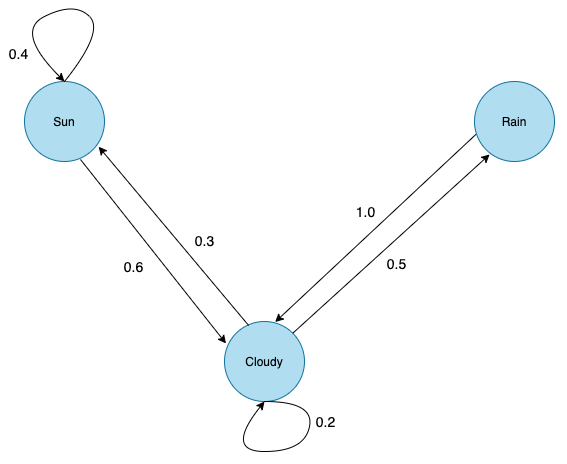
\includegraphics[scale=0.4]{markov_chain}
\caption{An example of a Markov Chain describing weather conditions.}
\label{fig:markov_chain}
\end{figure}
\hspace*{-1.5in}

While a graph representation of a Markov Chain is useful, in most cases it's convenient to think of it as a matrix.
Specifically, an element $0 \leq P_{ij} \leq 1$ of a matrix $P$ is defined as the probability of transitioning from
the state $i$ to the state $j$.\ As the $i$-th row of such matrix defines probabilities of transitioning from the
$i$-th  state to all other states, it holds $\sum_{j = 1}^{n} P_{ij} = 1$.\ A matrix with such properties is called a
$stochastic$ matrix.\ In the next sections, we will think of a Markov Chain as a $stochastic$ matrix.

\begin{definition}
A vector $\mu^{(0)} = (\mu^{(0)}_1, \mu^{(0)}_2, \dots, \mu^{(0)}_n)$ such that $\sum_{i=1}^{n} \mu^{(0)}_i = 1$
is called an $initial\ state$ of a Markov Chain.\ It defines an initial distribution across the state space.

\end{definition}

The Markov Chain process is fully characterized by a transition matrix $P$ and an initial state $\mu^{(0)}$.\ In
particular, the distribution of a Markov Chain in the $k$-th step can be uniquely determined by utilising the
formula $\mu^{(k)} = \mu^{(0)}P^k$.\ Although a Markov Chain can contain infinitely many states, we only consider
Markov Chains with a finite number of states.\ In particular, some theorems presented in the next sections
are not true without this assumption.\newline

\section{Stationary distribution}

In this section we will formalize a notion of a $stationary$ distribution and explore its properties.\ Furthermore,
we will provide sufficient conditions to guarantee that a Markov Chain has a unique $stationary$ distribution.

\begin{definition}
A vector $\pi = (\pi_1, \pi_2, \dots, \pi_n)$ is called a $stationary$ distribution iff $\pi P = \pi$, where $P$
denotes a transition matrix of a Markov Chain.
\end{definition}

One can convince yourself that a Markov Chain can have multiple $stationary$ distributions.\ An example of such Markov
Chain is when $P = Id$, which implies that any probability distribution is stationary.\ In the remaining part of this
section we will characterize a family of Markov Chains with a unique stationary distribution.

\begin{definition}
A Markov Chain with a transition matrix $P$ is called $irreducible$ iff for each pair of a source state $i$ and
a destination state $j$, it's possible to transition from $i$ to $j$ in a finite time i.e. there exists $k$ such that
$(P^k)_{ij} > 0$.
\end{definition}

\begin{definition}
A period of the $i$-th state is defined as $p(i) = gcd(\{n \geq 1 : (P^n)_{ii} > 0\}$.\ A state is called
$aperiodic$ iff $p(i) = 1$.\ A Markov Chain is called aperiodic if all of its states are aperiodic.
\end{definition}

A Markov Chain that respects the two above-mentioned properties is called an $ergodic$ Markov Chain.\ Interestingly,
$ergodic$ Markov Chains have many useful properties that leads to sophisticated algorithms.

\begin{theorem}\label{thm:one_stationary}
For any $ergodic$ Markov Chain, there exists exactly one stationary distribution $\pi$.
\end{theorem}

\begin{theorem}\label{thm:converges_to_stationary}
Let $\mu^{(0)}$ be an arbitrary initial state of any $ergodic$ Markov Chain.\ Let
$d_{TV}(\mu^{(n)}, \pi) = \frac{1}{2} \sum_{i = 1}^{k} |\mu_i^{(n)} - \pi_i|$ denote a distance between a
distribution of possible states in the $n$-th step and a stationary distribution of the defined Markov Chain.\ Then,
it holds $\lim_{n \to \infty} d_{TV}(\mu^{(n)}, \pi) = 0$.
\end{theorem}

The proofs on the theorems \ref{thm:one_stationary} and \ref{thm:converges_to_stationary} can be found in
\cite{markov_chains_book}.\ From the practical point of view, the presented theorems imply that an $ergodic$ Markov
Chain always converges to its stationary distribution, regardless of the initial distribution.\ Note that the
presented theorems do not guarantee any convergence speed.

\section{Reversible Markov Chains}

Reversible Markov Chains show up in many different areas e.g.\ they are the main building block for the Markov
Chain Monte Carlo methods.\ Formally, the reversed process is defined as $\tilde{X_t} = X_{T - t}$.\ Intuitively,
$\tilde{X}$ represents a Markov chain that is reversed in a time.

\begin{definition}
A probability distribution $\tilde{\pi}$ is said to be $reversible$ for a Markov Chain with a transition matrix $P$
iff for any $i,j$ it holds $\tilde{\pi_i} P_{ij} = \tilde{\pi_j} P_{ji}$.\ A Markov Chain is called a $reversible$
chain iff $\tilde{X_t} = X_t$ i.e. the reversed process is the same as the forward process.
\end{definition}

\begin{theorem}\label{reversible_chain}
A Markov Chain with a stationary distribution $\pi$ is reversible iff for any $i, j$ it holds
$\pi_i P_{ij} = \pi_j P_{ji}$.
\end{theorem}

The $Theorem$ \ref{reversible_chain} has many useful implications.\ First of all, in order to determine whether a
distribution is $reversible$, it suffices to check if it exists a probability measure $\tilde{\pi}$ such that
for any $i, j$ it holds $\tilde{\pi_i} P_{ij} = \tilde{\pi_j} P_{ji}$.\ What is more, in case we find such
$\tilde{\pi}$, it follows that $\pi = \tilde{\pi}$ i.e.\ the probability measure that we found is a stationary
distribution.\ This gives us a powerful tool for finding a stationary distribution.

\numberedchapter{Markov Chain Monte Carlo methods}

Consider a problem of sampling a random permutation from the set of $100$ elements.\ One can show that such space
contains $100!$ elements, implying that putting all permutations in the memory of a computer is not feasible.\ While
there exist algorithms for sampling permutations from a uniform distribution, the problem becomes harder in the case of
a skewed distribution.\ For instance, let our target distribution be defined based on positions of permutation's
elements e.g.\ $d(x) = \prod_{i = 1}^{n} e^{i * x_i}$, where $x_i$ denotes the $i$-th element of the permutation.\ While
the problem of sampling from such distribution can not be tackled using any trivial algorithm, it's possible to
simulate it with Markov Chains.\newline

In this chapter, we show how to deal with a situation in which we have a large state space and our task is to sample
an element from this space effectively.\ We will leverage the theory presented in the previous section to show how
to construct a Markov Chain with a stationary distribution equal to the target distribution we want to sample from.

\section{Metropolis–Hastings algorithm}

Let us denote the target distribution we want to sample from as $\tilde{\pi}$.\ Notice that in order to produce samples
from $\tilde{\pi}$ one may construct a Markov Chain $X$ with a transition matrix $P$ and a stationary distribution
$\pi = \tilde{\pi}$.\ Then, it suffices to simulate $X$ until we reach the stationary distribution.\ Assuming
that $X$ is $ergodic$, it can start in any initial state and based on $Theorem$ \ref{thm:converges_to_stationary} it
is guaranteed to converge to $\pi$.\ As one of our assumptions says that the space of states is very large,
constructing such Markov Chain explicitly does not solve our problem.\ Nevertheless, we can simulate such Markov Chain
with a Metropolis-Hastings algorithm.\newline

Before presenting the full algorithm, we will show how to construct a matrix $P$ such that $\tilde{\pi}$ is a
stationary distribution of a Markov Chain $X$ corresponding to $P$.\ Let us assume that we have some $proposal$
distribution $Q$ that defines a transition matrix of a Markov Chain with the same state space as $X$.\ Going further,
let us define a matrix $P$ by the following formula:\newline
$$
P_{ij} =
\begin{cases}
  Q_{ij}\min{(1, \frac{\pi_j Q_{ji}}{\pi_i Q_{ij}})} &\text{if $i \ne j$}\\
  1 - \sum\limits_{k \ne i}Q_{ik} \min{(1, \frac{\pi_k Q_{ki}}{\pi_i Q_{ik}})} &\text{otherwise}
\end{cases}
$$

While at first it may be unintuitive why $P$ would have a stationary distribution $\pi$, it can be easily
proved.\ To do so, let us show that for any $i, j$ it holds $\pi_i P_{ij} = \pi_j P_{ji}$.\ Without any loss of
generality, we can assume that $\frac{\pi_j Q_{ji}}{\pi_i Q_{ij}} \leq 1$, which implies that
$\frac{\pi_i Q_{ij}}{\pi_j Q_{ji}} \geq 1$.\ Putting everything together, we get
$$
\pi_i P_{ij} = \pi_i Q_{ij} \frac{\pi_j Q_{ji}}{\pi_i Q_{ij}} = \pi_j Q_{ji} = \pi_j P_{ji}
$$
which proves that $\pi_i P_{ij} = \pi_j P_{ji}$.\ The case when $\frac{\pi_j Q_{ji}}{\pi_i Q_{ij}} \geq 1$ is
symmetric.\ Using the $Theorem$ \ref{reversible_chain}, we can conclude that $\pi$ is the stationary distribution of
the constructed Markov Chain.\newline

Equipped with the method for generating a transition matrix $P$ for a given stationary distribution $\pi$, one may
construct an algorithm \ref{alg:metropolis_hastings} simulating a Markov Chain that corresponds to $P$.\ In case the
proposal distribution $Q$ is symmetric (i.e.\ $Q_{ij} = Q_{ji}$), the presented algorithm is called the $Metropolis$
algorithm, while in the general case of non-symmetric $Q$ it is called the $Metropolis$-$Hastings$ algorithm.\newline


\begin{algorithm}[tb]
\caption{Metropolis-Hastings}\label{alg:metropolis_hastings}
\begin{algorithmic}[1]
\State{\textbf{Input:} proposal distribution $Q$}
\State{\textbf{Input:} the current state $X_n = i$, where $n$ denotes the latest step of the simulation}
\State{Sample $j$ from a distribution $Q_i = (Q_{i1}, Q_{i2}, \dots, Q_{iN})$}
\State{Let $p = \min{(1, \frac{\pi_j Q_{ji}}{\pi_i Q_{ij}})}$}
\State{Sample $U \sim Unif(0, 1)$}
\If{$U \leq p$}
    \State{Set $X_{n + 1}$ = j}
\Else
    \State{Set $X_{n + 1} = X_n$}
\EndIf
\State{\textbf{Output:} the next state $X_{n + 1}$}
\end{algorithmic}
\end{algorithm}

\section{Gibbs sampling}

In this section we will show how to simulate Markov Chains for some specific distributions.\ Specifically, let us assume
that each possible state in a given state space can be represented by a function $e_i : V \to S$ that maps each vertex
$v \in V$ of an underlying graph $G = (V, K)$ to one of possible values $s \in S$.\ Generally, a state that is
represented in this form is often called a $configuration$.\ While for some distributions this
representation may not make sense, there are multiple cases for which it is the most natural way of expressing a
given distribution.\ For instance, consider a problem of colouring a graph.\ In this case, each state corresponds to a
possible graph colouring i.e.\ each vertex $v \in V$ has assigned one colour $s \in S$.\ Note that as in the graph
colouring problem it is required that two adjacent vertices are not assigned the same colour, some configurations
are not allowed.\newline

Now, assume that we are given a function $H : e \to \mathbb R_{\geq 0}$ that assigns an unnormalised probability to
each configuration $e \in E$.\ Our goal is to sample configurations according to the probabilities defined by the
function $H$.\ Let us show how to simulate a Markov chain satisfying this condition.\ To perform the $(k + 1)$-th
step of the algorithm, assuming that the current state is equal to $X_k = e_i$, first draw a vertex $\tilde{v} \in V$
uniformly and for each $s \in S$ calculate the probability
$$
P(e_{\tilde{v}} = s | e_{-\tilde{v}} = e_i) = \frac{\pi_{e_{\tilde{v}} =
s,e_{-\tilde{v}} = e_i}}{\sum_{s' \in S} \pi_{e_{\tilde{v}} = s', e_{-\tilde{v}} = e_i}}
$$

where $e_{\tilde{v}}$ denotes $s \in S$ corresponding to the vertex $\tilde{v} \in V$ and $e_{-\tilde{v}}$
denotes assignments of $s \in S$ to  all vertices $v \in V$ with $\tilde{v}$ excluded.\ The last step of the algorithm
involves sampling $\tilde{s} \in S$ from the probability distribution $P(e_{\tilde{v}} = s | e_{-\tilde{v}} = e_i)$
and setting
$$
X_{k + 1}(v) =
\begin{cases}
  \tilde{s} &\text{if $v = \tilde{v}$}\\
  X_k(v) &\text{otherwise}
\end{cases}
$$

The presented $Gibbs$ sampling algorithm is a special case of the $Metropolis$-$Hastings$ algorithm with the proposal
distribution
$$
Q_{ij} =
\begin{cases}
  \frac{1}{Z} &\text{iff $i$ is adjacent to $j$}\\
  0 &\text{otherwise}
\end{cases}
$$

which provides an instant proof of the the fact that the presented algorithm simulates a Markov Chain with the
stationary distribution $\pi$.\ An alternative proof of this fact can be found in \cite{mcmc_book}.\ The advantage of
the $Gibbs$ algorithm over the $Metropolis$-$Hastings$ algorithm is that it avoids constructing  the proposal
distribution $Q$.\ At the same time, for some cases the lack of control over $Q$ is a major downside as we will see
in the following chapters.

\numberedchapter{Ising model and its applications}

TODO

\section{Formal definition of the Ising model}

TODO

\section{Application to binary image denoising problem}

TODO

\section{Extension to grayscale images}

TODO

\section{Applying MCMC methods to the Ising model}

TODO

\numberedchapter{Gradient-based image denoising}

TODO

\section{Proposal distribution inspired by gradients}

TODO

\section{Efficient implementation for image denoising problem}

TODO

\numberedchapter{Experiments: binary images}

TODO

\section{Methodology}

TODO

\section{Denoising quality based on image size}

TODO

\section{Denoising quality based on noise level}

TODO

\section{Sensitivity of noise level prior parameter}

TODO

\section{Qualitative results}

TODO

\numberedchapter{Experiments: grayscale images}

TODO

\section{Methodology}

TODO

\section{Denoising quality}

TODO

\section{Qualitative results}

TODO

\numberedchapter{Summary}

TODO

Podstawowym problemem, z jakim zmagają się wszyscy przedsiębiorcy, jest przygotowa- nie oferty w ten sposób, by była ona zarówno atrakcyjna dla klienta (a przynajmniej bardziej atrakcyjna niż to, co oferuje konkurencja), jak i przynosiła zyski dla przedsiębiorcy (a już na pewno nie generowała strat). Branża ubezpieczeniowa nie jest tu wyjątkiem. Każda ubez- pieczalnia zatrudnia sztab aktuariuszy, których zadaniem jest wyznaczenie obowiązkowych składek w ten.
Computers \cite{einstein} sdsd.
Podstawowym problemem, z jakim zmagają się wszyscy przedsiębiorcy, jest przygotowa- nie oferty w ten sposób, by była ona zarówno atrakcyjna dla klienta (a przynajmniej bardziej atrakcyjna niż to, co oferuje konkurencja), jak i przynosiła zyski dla przedsiębiorcy (a już na pewno nie generowała strat). Branża ubezpieczeniowa nie jest tu wyjątkiem. Każda ubez- pieczalnia zatrudnia sztab aktuariuszy, których zadaniem jest wyznaczenie obowiązkowych składek w ten sposób, by pokryły koszta działalności firmy oraz przyszłe zobowiązania wzglę- dem klientów. W przypadku ubezpieczeń majątkowych zadanie jest o tyle trudniejsze, że bardzo istotny jest tak zwany czynnik ludzki czyli np. skłonność do ryzyka lub umiejętność prowadzenia pojazdów. Są to parametry trudne do zmierzenia, stąd potrzeba jak najlepsze- go modelowania wpływu tych składowych na wartość zgłaszanych szkód, na skutek których konieczna będzie wypłata odszkodowania. Obecnie najczęściej stosowaną metodą jest sys- tem Bonus - Malus, którego głównym założeniem jest związanie wysokości składki z liczbą wypadków spowodowanych przez kierowcę. Wadą tego rozwiązania jest nieuwzględnianie istot- nych czynników takich jak np. częstotliwość prowadzenia pojazdu czy styl jazdy. Pomysłem na rozwiązanie tego problemu jest montowanie w samochodach urządzeń rejestrujących jaz- dę, jednak może się to spotkać z oporem klientów dbających o ochronę swojej prywatności. Powstaje więc pytanie jak poprawić stosowane rozwiązania bez konieczności zbierania dodat- kowych danych o kierowcy. Odpowiedzią na to pytanie mogą być tak zwane ukryte modele Markowa.
Figure \ref{fig:xxx} compared with Figure \ref{fig:yyy} sss \cite{einstein} sdsd.


\begin{figure}
\centering
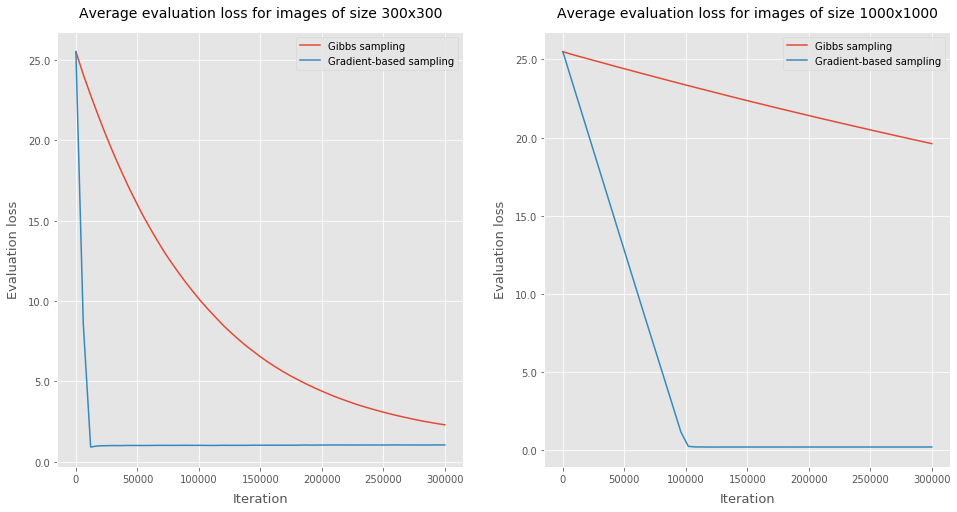
\includegraphics[scale=0.4]{binary_input_size_plots}
\caption{Example of a parametric plot ($\sin (x), \cos(x), x$)}
\label{fig:xxx}
\end{figure}
\begin{figure}
\centering
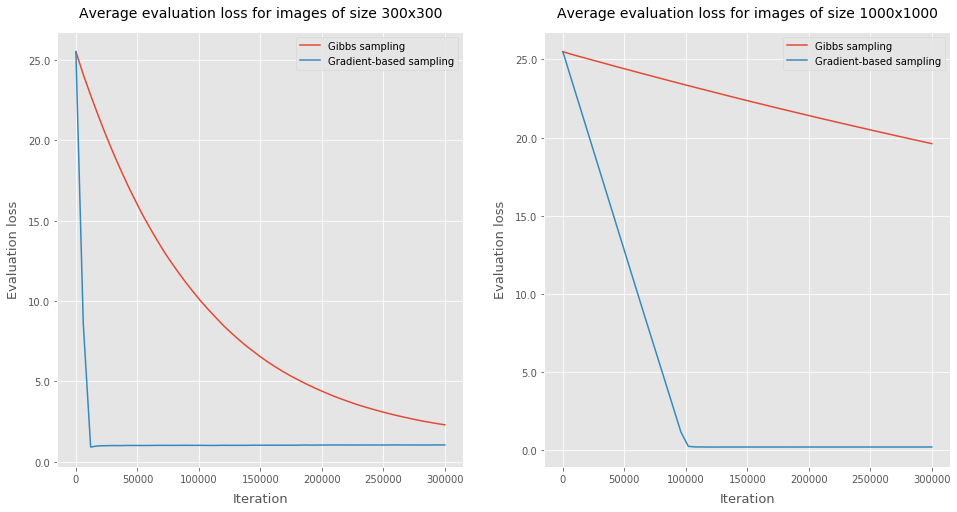
\includegraphics[scale=0.4]{binary_input_size_plots}
\caption{Example of a parametric plot ($\sin (x), \cos(x), x$)}
\label{fig:yyy}
\end{figure}

\begin{thebibliography}{9}

\bibitem{markov_chains_book}
Olle Häggström - \textit{Finite Markov chains and algorithmic applications (2002)}

\bibitem{mcmc_book}
Pierre Bremaud - \textit{Markov Chains: Gibbs Fields, Monte Carlo Simulation, and Queues (1999)}

\end{thebibliography}

\end{document}
